With data aggregation rapidly growing in volume over the last few decades, it becomes increasingly more difficult to process gathered data into insightful information.
We are now exploring first cognisances in the field of dimensionality reduction and are then going to summarise underlying theories to be able to better grasp and tackle this problem.

\vfill


%%%%%%%%%%%%%%%%%%%%%%%%%%%%%%%%%%%%%%%%%%%%%%%%%%%%%%%%%%%%%%%%%%%%%%%%%%%%%%%

\subsection{Necessity}
The necessity of reducing dimensions in a large data set serves different purposes in the problems we face in data science. 
Now follows a summary of the different applications where we can utilise the methods of dimensionality reduction. 
Finally, we will conclude how despite their disparities, the various application methods come together in our goal of finding tractable and resource-conscious solutions.
\vspace{-5mm}

\paragraph{Computational impact}

The most intuitive benefit is certainly its impact on computational performance.
Having fewer features reduces our required storage space and allows our learning algorithms to run much faster. \cite{PythonMachineLearningCh1}
\vspace{-5mm}

\paragraph{Feature engineering}

Our models will only be capable of producing relevant results if the features we supply it with are also relevant. \cite{HandsOnMLCh1}
\emph{Feature extraction} combines many semantically related features into few, which are found through dimensionality reduction. 
This helps us to reduce the number of features while retaining as much information as possible from the originating data set.
This is not to be confused with \emph{feature selection}, which does not benefit from dimensionality reduction and is therefore not considered in this work.
\vspace{-5mm}

\paragraph{Data visualisation}

Reducing dimensions can also help us to visually represent data in an intuitive fashion.
Even picturing a relatively basic 4-dimensional hypercube is incredibly difficult to make sense of.
Actively recalling this information is not only important for our own understanding of data. It is even more important when sharing our observations and ideas with other data scientists and essential when communicating our conclusions to people in an interdisciplinary environment. \cite{PythonMachineLearningCh5}
\vspace{-5mm}

% \paragraph{Traceability}

% Having discussed the importance of understanding the problem and its solution earlier in section \ref{curseOfDimensionality}, it is often important to be able to comprehend the prediction a model makes instead of trusting a black box model. 
% Reducing the dimensions and understanding the given data helps us to alleviate this issue.
% \vspace{-5mm}

\paragraph{Conclusion}

Considering the computational impact helps us to narrow down a complex task into a feasible scope to find resource-conscious solutions.
Feature extraction helps us to remove dimensions coupled with an increase in predictive performance right off the bat.
This helps us to visualise the data and to be able to understand and trace its predictions.
Combined, this helps us to build a tractable solution to our problem.

\clearpage



%%%%%%%%%%%%%%%%%%%%%%%%%%%%%%%%%%%%%%%%%%%%%%%%%%%%%%%%%%%%%%%%%%%%%%%%%%%%%%%

\subsection{Mathematical background}
To round up the theoretical premises required for this topic, we will become aware of the boundaries of intuitive mathematical concepts which result in highly counter-intuitive behaviours in high-dimensional space.

\subsubsection{Euclidean distance \& sparse matrices}

An important aspect which is frequently utilised in various machine learning methods is to evaluate the Euclidean distance between two points in a high-dimensional space.
While the concept is simple to understand and illustrate in two or three dimensions, its behaviour in a high-dimensional space changes dramatically and it becomes heavily counter-intuitive to get a hold off.

Most notably, if you pick two random points in a unit \gls{hypercube}, the higher the dimensions, the higher the average distance between these two points will be \cite{HandsOnMLCh8}.
This implies that, the higher the dimensionality of a data set, the higher the chance of overfitting.
In this scenario, matrices which represent a high-dimensional data set with distant entries are called sparse matrices.

\vspace{2mm}



\subsubsection{Eigenvalues and eigenvectors}

The theories behind eigenvalues and eigenvectors are utilised extensively in \acrlong{dr}.
Due to this, we will quickly recall the key concepts behind the eigenvalue equation $A \overrightarrow{x} = \lambda \overrightarrow{x}$:


\begin{itemize}
	\item Eigenvalues and eigenvectors only apply to squared matrices.
	\item When searching for an eigenvalue $\lambda$, we subtract $\lambda$ along the main diagonal of a matrix $A$ such that $A - \lambda I$ is \gls{singular} ($I$ being the identity matrix) \cite{Strang2005tn}.
	\item The entire factorisation looks as following:
	\begin{align}
		\label{formula:eigenONE}
		A \overrightarrow{x} &= \lambda \overrightarrow{x} 
		\\
		%
		\label{formula:eigenTWO}
		A \overrightarrow{x} &= (\lambda I) \overrightarrow{x}
		\\
		%
		\label{formula:eigenTHREE}
		A \overrightarrow{x} - (\lambda I) \overrightarrow{x} &= 0
		\\
		%
		\label{formula:eigenFOUR}
		(A - \lambda  I) \overrightarrow{x} &= 0
		%
	\end{align}
	\item \reff{eigenTWO} translates the scalar-vector multiplication into a matrix-vector multiplication.
	\item $\overrightarrow{x} = \overrightarrow{0}$ is not semantically relevant and therefore not considered.
\end{itemize}

% \begin{itemize}
% 	\item Only square matrices have eigenvectors and eigenvalues
% 	\item We will make heavy use of transposing matrices
% 	\item Identity matrix, Properties of diagonal matrices, General formula
% 	\begin{align}
% 		\label{formula:one}
% 		A \cdot x &= \lambda \cdot x 
% 		\\
% 		%
% 		\label{formula:two}
% 		A \cdot x &= \lambda \cdot x \cdot I
% 		\\
% 		%
% 		\label{formula:three}
% 		(A - \lambda \cdot I)\cdot x &= 0
% 		%
% 	\end{align}
% \end{itemize}

% \reff{one}

% \reff{two}

% \reff{three}



%%%%%%%%%%%%%%%%%%%%%%%%%%%%%%%%%%%%%%%%%%%%%%%%%%%%%%%%%%%%%%%%%%%%%%%%%%%%%%%

\subsection{The curse of dimensionality} \label{curseOfDimensionality}
The concept of the \emph{curse of dimensionality} was first introduced by Richard Bellman in 1957 \cite{DynProg}.
His book, \emph{Dynamic Programming}, explains a method he has developed to explore more efficient solutions to counteract the increasing complexity in problems facing our day-to-day lives. 
The range of domains where applicable is vast and even covers problems that were impossible to foresee for Richard Bellman.
Most notable to us, this includes data science in the 21st century and falls right into the realm of \acrlong{dr}.
\bigskip

Bellman observed that, when considering a larger set of variables, even simple and well-understood problems such as determining the maximum of a given function becomes worrisome.
Large data sets face a variety of difficulties of both obvious and subtle nature.

The obvious issues primarily consist of a finite number of computational resources available, especially back in the 1950s. 
Having access to the computer systems we have today, they could certainly be considered a computational nirvana for any scientists and mathematicians 65 years ago.
While Bellman fantasised about such possibilities, he proactively considered them and accurately thought of more subtle problems that could potentially arise.
His observations were spot on and are an important factor in why his theories are still as relevant as ever nowadays.

\emph{The problem is not to be considered solved in the mathematical sense until the structure of the optimal policy is understood} \cite{DynProg}.
This quote from Richard Bellman eloquently summarises the problem at hand.  
While it appears plausible, that more quantitative measurements would yield more accurate predictions, our extremely complicated world often misleads us.
This results in ourselves neither being able to rigorously understand the problem, nor to improve our predictions of challenges we are unable to analyse.
We need to walk a narrow path between the \emph{Pitfalls of Oversimplification and the Morass of Overcomplication} \mycite{DynProg}.
\bigskip

With the premise being described by Bellman in 1957, we can conclude that many features do not only heavily impede model training but can additionally result in worse solutions \cite{HandsOnMLCh8}.
Simulteneously when considering the performance and traceability aspects.

\vfill
\clearpage

%%%%%%%%%%%%%%%%%%%%%%%%%%%%%%%%%%%%%%%%%%%%%%%%%%%%%%%%%%%%%%%%%%%%%%%%%%%%%%%

\subsection{Linear vs. Non-linear methods}
The utmost category, used to differentiate between various techniques is fortunately mutually exclusive to any method.
Thanks to this characteristic, we can distinctively classify, and associate a given technique.
This allocation, contrary to the following classifications, is the one that considers the domain of the problem.

Thus, it requires special attention by its users since it can easily be used erroneously.
We need to understand the gross patterns in the data set we need to operate on.
\medskip

The below figure \ref{fig:linearvsnonlinearproblems} illustrates and contrasts the general patterns that we need to identify:\vspace*{4mm}

\renewcommand{\tikzscale}{1.18}
\begin{figure}[h]
	\begin{subfigure}{0.48\textwidth}
	    \caption{Linear problems}
		\begin{tikzpicture}[scale=\tikzscale]
	% AXIS
	\draw[->,ultra thick,color=pptAccentII]
		(0,0)--(5,0) 
			node[midway, below,yshift=-1mm]{$x_1$};

	\draw[->,ultra thick,color=pptAccentII] 
		(0,0)--(0,5) 
			node[midway, left, xshift=-1mm]{$x_2$};

	% DIAGONAL LINE
	% \draw[-, dashed,color=pptAccentII] 
		% (0.2,0.2)--(4.5,4.5)
				% ;

	% NODES

	\begin{scope}[color=pptAccentIII,line width=1.25pt]
	 	\newcommand{\lowerarray}{%
	 		{2.3,1.7},{3.3,0.7},{1.2,0.5},{2.7,1.2},{2.4,1.4},{1.8,1.2},{3.4,2.4},{3.2,0.5},{1.3,0.7},{1.2,0.7},{3.7,1.8},{3.5,0.6},{2.4,0.6},{3.3,2},{1.5,0.9},{1.3,0.8},{1.3,0.7},{3.6,0.6},{3.2,2},{3.8,1.7},{1,0.5},{2.8,0.6},{3.9,2.5},{2.6,0.9},{3.7,1.7},{2.3,0.6},{3.9,1.4},{3.8,2.5},{1.4,0.7},{1.7,0.9},{3,2.4},{1.9,0.8},{2,1.5},{2.4,1.6},{1.4,0.9},{1.9,0.9},{2.8,1.7},{1.6,0.5},{3.9,0.8},{3.9,1.8},{2.3,0.7},{2.5,1.6},{1.4,0.7},{4,3.5},{3.1,0.9},{3.4,2.5},{3.3,2.2},{4,1.5},{2,1.5}%
	 	}

		\foreach \i in \lowerarray {
		 	\draw (\i) 
		 		circle (2pt);
		}
 	\end{scope}

	\begin{scope}[color=pptAccentIV,line width=1pt]
	 	\newcommand{\upperarray}{%
	 		{2.9,4},{1.7,2.7},{3.2,3.8},{2.6,3.8},{2.5,3},{3.5,4.5},{2.3,4.2},{2.8,4.3},{2.5,4.2},{4,4.5},{3.6,4.2},{3.8,4.5},{4,4.5},{1.4,4.1},{3.6,4.1},{1.2,3.7},{3.7,4.2},{3.5,4.4},{1.7,4.1},{2.3,4},{2.2,2.7},{1.4,4.2},{2.3,3.7},{4,4.5},{2.6,3.8},{1.9,2.4},{3.3,4.3},{2.8,4.4},{1.8,2.8},{1,3.1},{2.1,4.4},{1.2,3.7},{4,4.5},{2.2,3.5},{3.5,4.3},{1,1.5},{1.2,3.1},{2.2,2.9},{1.8,2.3},{1.4,4.1},{3.7,4.3},{3,3.9},{3.4,4},{1.8,3.7},{1.8,4.3},{2.5,4},{3.7,4.4},{2.8,3.8},{1.5,4.1}%
	 	}

		\foreach \i in \upperarray {
		 	\node[isosceles triangle,draw,isosceles triangle apex angle=60,rotate=90, minimum size=3pt,inner sep=0pt] (T) at (\i){};
		}

	 \end{scope}

\end{tikzpicture}

	    \label{subfig:linearproblems}
	\end{subfigure}
	\hfill
	\begin{subfigure}{0.48\textwidth}
	    \caption{Non-linear problems}
		\begin{tikzpicture}[scale=\tikzscale]
	% AXIS
	\draw[->,ultra thick,color=pptAccentII] 
		(0,0)--(5,0) 
			node[midway, below, yshift=-1mm]{$x_1$};

	\draw[->,ultra thick,color=pptAccentII] 
		(0,0)--(0,5) 
			node[midway, left, xshift=-1mm]{$x_2$};

	% DELIMITER CIRCLE
 	% \draw (2.5,2.5)[dashed,color=pptAccentII]
 		% circle (42pt);

	% NODES

	\begin{scope}[color=pptAccentIII,line width=1.25pt]
	 	\newcommand{\innerarray}{%
	 		{2.4,2.5},{1.8,1.8},{3,3.4},{3.4,2.1},{1.9,2.8},{1.6,2.1},{2,1.6},{2.7,2.7},{3,3.5},{3,2.4},{2.6,1.5},{2,2.6},{2.7,3},{1.5,3},{2.6,2.7},{3.1,2},{1.9,3.4},{2,2.6},{3,2.2},{1.6,3.2},{2.8,1.5},{2.3,2.7},{2.6,2.5},{2.5,3.5},{3.3,1.7},{2.1,1.8},{2.2,2.1},{1.6,2.8},{3.1,2.9},{1.7,2.2},{1.6,2.9},{2.7,2.7},{2,1.8},{3,1.7},{3.4,2.7},{3.4,2.3},{2.1,2.6},{1.7,1.7},{2.9,3.2},{1.6,3},{3,2.9},{2.4,2.6},{2.5,2.8},{3.3,3.2},{2.9,2.2},{2.3,2.2},{2.8,2.7},{2,2.5},{3.1,1.8}%
	 	}

		\foreach \i in \innerarray {
		 	\draw (\i) 
		 		circle (2pt);
		}
 	\end{scope}

	\begin{scope}[color=pptAccentIV,line width=1pt]
	 	\newcommand{\outerarray}{%
	 		{0.2,0.6},{0.9,0.9},{1.3,0.4},{0.4,0.5},{0.7,1.1},{1.2,0.2},{1.3,0.4},{0.3,0.4},{0.5,1.4},{0.9,1.2},{0.5,0.4},{0.3,0.3},{4.3,4.3},{4.5,4.1},{4.2,4.5},{3.9,4.4},{3.7,4.5},{3.9,3.7},{4.4,4.1},{4.2,4.4},{3.9,3.7},{3.9,4},{3.8,3.6},{4,4},{4.4,0.6},{4.1,1.4},{3.7,1.1},{3.9,0.6},{4.3,0.3},{4.2,1.4},{4.2,0.7},{3.8,1.3},{4.1,0.7},{4.1,1.1},{4.3,1.2},{4.3,1.4},{0.2,4.5},{1.1,4.3},{1.2,4.5},{0.8,3.6},{0.8,3.6},{0.4,4.2},{0.5,4.2},{0.8,3.7},{0.2,3.5},{0.4,4.3},{0.9,3.8},{0.5,4.5},{3.2,0.8},{3.5,0.8},{3.3,0.8},{2.7,0.8},{2.1,0.5},{2.3,0.6},{2,0.6},{3.4,0.8},{3.1,0.5},{2.7,0.8},{3.5,0.7},{2.6,0.5},{0.8,3.1},{0.7,2.4},{0.7,3.1},{0.8,2.6},{0.6,2.1},{0.5,2.9},{0.8,2.2},{0.7,2.9},{0.8,2.4},{0.7,3.1},{0.8,3.4},{0.7,2.2},{3.4,4.4},{2.8,4.2},{2.4,4.5},{3.5,4.5},{3.4,4.2},{3.1,4.5},{2.9,4.3},{2.5,4.5},{3.4,4.5},{2.2,4.2},{3.1,4.5},{2.7,4.5},{4.5,3},{4.5,2.7},{4.3,2.3},{4.2,2.3},{4.2,2.9},{4.5,2.5},{4.2,2.6},{4.4,2.1},{4.2,2.1},{4.2,2},{4.3,3.4},{4.4,2.2}%
	 	}

		\foreach \i in \outerarray {
		 	\node[isosceles triangle,draw,isosceles triangle apex angle=60,rotate=90, minimum size=3pt,inner sep=0pt] (T) at (\i){};
		}

	 \end{scope}

\end{tikzpicture}

	    \label{subfig:nonlinearproblems}
	\end{subfigure}
\caption{Linear vs. non-linear problems.}
\label{fig:linearvsnonlinearproblems}
\end{figure}

As we can see in figure \ref{subfig:linearproblems}, a linear problem is given when we are able to identify a straight line, or any \gls{hyperplane}, to split the data into unambiguous subsets.
Intuitively and, as we will later examine, factually, these types of problem are comparably easy to solve.

A non-linear problem, as pictured in figure \ref{subfig:nonlinearproblems}, already looks more complex on the first glance.
And indeed, we will illuminate the solution approaches to this scenario and elaborate on its comportment.

\clearpage

%%%%%%%%%%%%%%%%%%%%%%%%%%%%%%%%%%%%%%%%%%%%%%%%%%%%%%%%%%%%%%%%%%%%%%%%%%%%%%%

\subsection{Projection vs. manifold learning}
% taken from ch 8 in géron's book

In this section, we will compare the general solution approaches available which can be utilised to solve both linear as well as non-linear problems. \cite{HandsOnMLCh8}

\todo{Not quite true, revisit this. \cite{Lee2007NonlinearDR} cite this.}

\renewcommand{\tikzscale}{0.33}
\begin{wrapfigure}[13]{r}{0.62\textwidth}
	\vspace*{-8mm}
	\centering
	\newcommand{\textproperties}[1]{\textcolor{gray}{\textbf{#1}}}
\newcommand{\circlecolor}{hkaRed}
\newcommand{\circlesize}{6}


%%%%%%%%%%%%%%%%%%%

\begin{tikzpicture}[scale=\tikzscale]
 	\node at (12.5,7) {\textproperties{example data set in 2D space:}};
	% AXIS
	\draw[->,ultra thick] 
		(0,0)--(25,0) 
			node[midway, below, yshift=-1mm]{$x$};

	\draw[->,ultra thick] 
		(0,0)--(0,5) 
			node[midway, left, xshift=-1mm]{$y$};

	% NODES

	\begin{scope}[color=\circlecolor]
	 	\newcommand{\datapoints}{%
	 		{24,1},	{23,1},	{21,3},	{4,2},	{8,1},	{20,2},	{19,1},	{17,2},	{7,2},	{24,1},	{5,2},	{2,3},	{5,2},	{9,1},	{24,1},	{14,2},	{12,2},	{12,1},	{17,1},	{24,2},	{12,2},	{18,2},	{18,1},	{12,1},	{10,3},	{24,2},	{24,3},	{22,1},	{9,2},	{16,2}%
	 	}

		\foreach \i in \datapoints {
		 	\filldraw (\i) 
		 		circle (\circlesize pt);
		}
 	\end{scope}

%%%%%%%%%%%%%%%%%%%

	\draw[->,ultra thick] (0,-6)--(25,-6);
 	\node at (12.5,-4) {\textproperties{projection on x \gls{hyperplane}:}};
	\node at (1,-7) {$x$};

	\begin{scope}[color=\circlecolor]
	 	\newcommand{\datapoints}{%
	 		{24,-6},	{23,-6},	{21,-6},	{4,-6},	{8,-6},	{20,-6},	{19,-6},	{17,-6},	{7,-6},	{24,-6},	{5,-6},	{2,-6},	{5,-6},	{9,-6},	{24,-6},	{14,-6},	{12,-6},	{12,-6},	{17,-6},	{24,-6},	{12,-6},	{18,-6},	{18,-6},	{12,-6},	{10,-6},	{24,-6},	{24,-6},	{22,-6},	{9,-6},	{16,-6}%
	 	}

		\foreach \i in \datapoints {
		 	\filldraw (\i) 
		 		circle (\circlesize pt);
		}
 	\end{scope}

%%%%%%%%%%%%%%%%%%%

 	\node at (12.5,-10) {\textproperties{projection on y \gls{hyperplane}:}};
	\draw[->,ultra thick] (0,-12)--(25,-12);
	\node at (1,-13) {$y$};

	\begin{scope}[color=\circlecolor]
	 	\newcommand{\datapoints}{%
	 		{6,-12},	{6,-12},	{18,-12},	{12,-12},	{6,-12},	{12,-12},	{6,-12},	{12,-12},	{12,-12},	{6,-12},	{12,-12},	{18,-12},	{12,-12},	{6,-12},	{6,-12},	{12,-12},	{12,-12},	{6,-12},	{6,-12},	{12,-12},	{12,-12},	{12,-12},	{6,-12},	{6,-12},	{18,-12},	{12,-12},	{18,-12},	{6,-12},	{12,-12},	{12,-12}%
	 	}

		\foreach \i in \datapoints {
		 	\filldraw (\i) 
		 		circle (\circlesize pt);
		}
 	\end{scope}


\end{tikzpicture}

	\captionsetup{justification=centering}
	\caption{Simple example of a projection}
    \label{fig:projectionExample}
\end{wrapfigure}

\paragraph{Projection} In contrast, this is the trivial concept of the two. The idea is to project the data points onto a \gls{hyperplane} which summarises the data with as little information loss as possible.

Figure \ref{fig:projectionExample} illustrates this in a simple example.
As we can observe, when we pick the right \gls{hyperplane}, such as the x axis in the example, we lose far fewer information than if we would have picked the y axis.


\paragraph{Manifolds} This concept is significantly more difficult to get a hold of.
Significant breakthroughs \cite{ma2012manifold} in this field were accomplished in the year 2000 in the significant and commonly cited paper \emph{A global geometric framework for nonlinear dimensionality reduction}. \cite{tenenbaum2000global}
To understand the basic idea, we will demonstrate its behaviour to get an idea of the problem using the popular swiss roll data set pictured in figure \ref{fig:swissrollfull}.


\noindent
\begin{minipage}[c]{0.4\linewidth}
%
\vspace*{6mm}
\begin{center}
	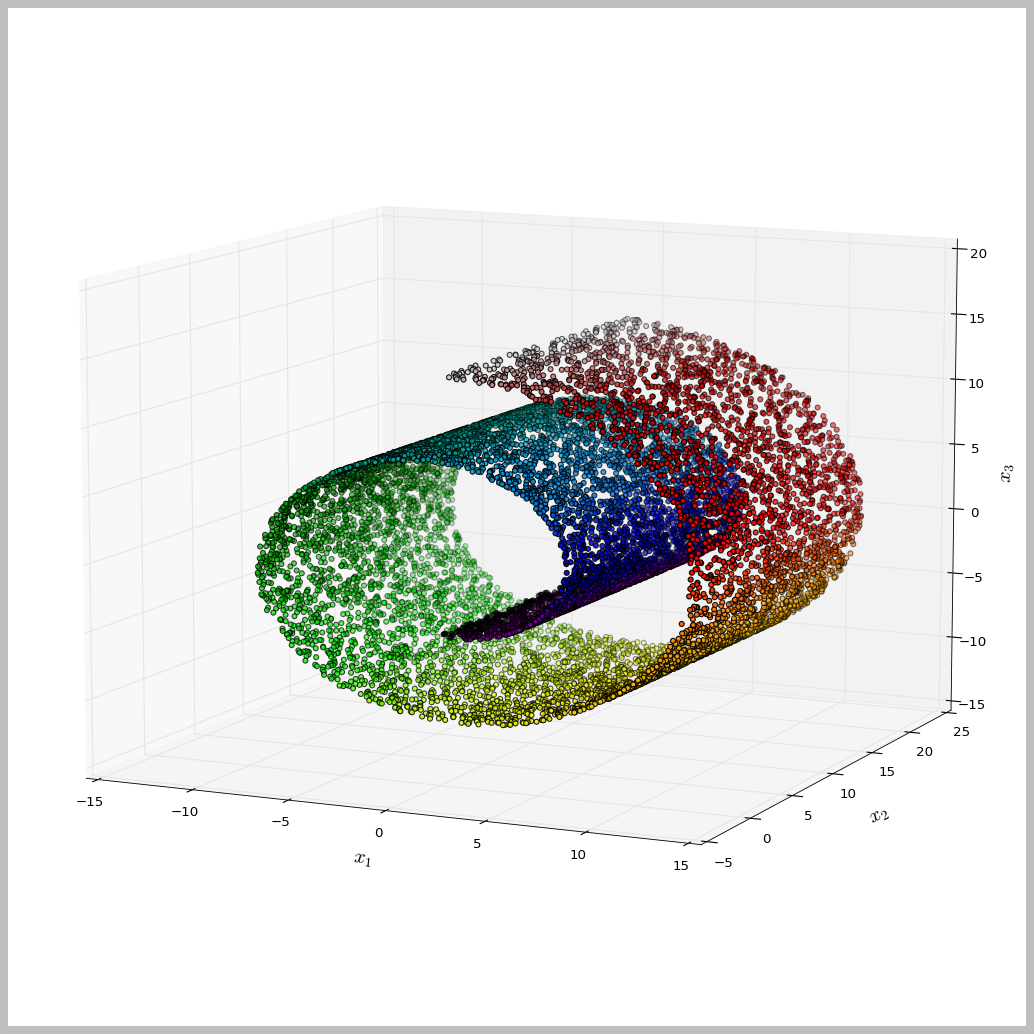
\includegraphics[width=0.9\textwidth]{external_content/graphs/swiss_roll.png}
	\captionsetup{justification=centering,type=htypei}
	\captionof{figure}{Swiss Roll generated from scikit-learn \cite{scikit-learn}}
	\label{fig:swissrollfull}
\end{center}
%
\end{minipage}\hfill%
\begin{minipage}[c]{0.55\linewidth}
Before demystifying this problem, we will then dive into various methods how to bend and twist high-dimensional data into lower-dimensional spaces.

Our goal is to avoid confusing projections such as shown in figure \ref{fig:swissrollprojection}:

\begin{center}
	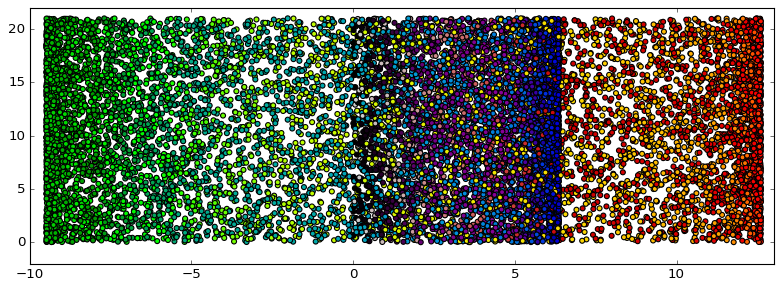
\includegraphics[width=0.8\textwidth]{external_content/graphs/swiss_roll-projection.png}
	\captionsetup{justification=centering,type=htypei}
	\captionof{figure}{Representation in 2D\\ of a projected swiss role}
	\label{fig:swissrollprojection}
\end{center}
\end{minipage}%

\clearpage
